\section{Dynamic Provisioning of Web Services for Simulation Workflows}
\label{previous:dynamic}

\citeauthor*{provisioning:dynamic} found some problems with the architecture proposed in \autoref{previous:ondemand}~\autocite{provisioning:dynamic}.
The original architecture assumes that only one provisioning engine is used at a time.
It neglects situations where services might require another (or multiple other) provisioning engines because their provisioning descriptions are not available in a format that the currently used provisioning engine understands.
It also assumes that the ESB communicates directly with this provisioning engine to deploy and undeploy other services.
This implicates that the ESB understands all manner of interfaces provided by various provisioning engines~\autocite{provisioning:dynamic}.

It further assumes that every provisioning engine knows how to communicate with the service repository to get the information and resources it needs to provision a service.
While this might be true for some provisioning engines, it is certainly not true for all of them.
This problem is further amplified because there are no standards defined for such a service repository~\autocite{provisioning:dynamic}.

Another assumption of the original architecture is that a provisioning engine always understands the format of the service packages provided by the service repository.
Different provisioning engines use different formats which are in general not compatible.
If provisioning engines would all use a standardized format (like CSAR), this would not be a problem, but that is not the case~\autocite{provisioning:dynamic}.

\begin{figure}[!htbp]
	\centering
	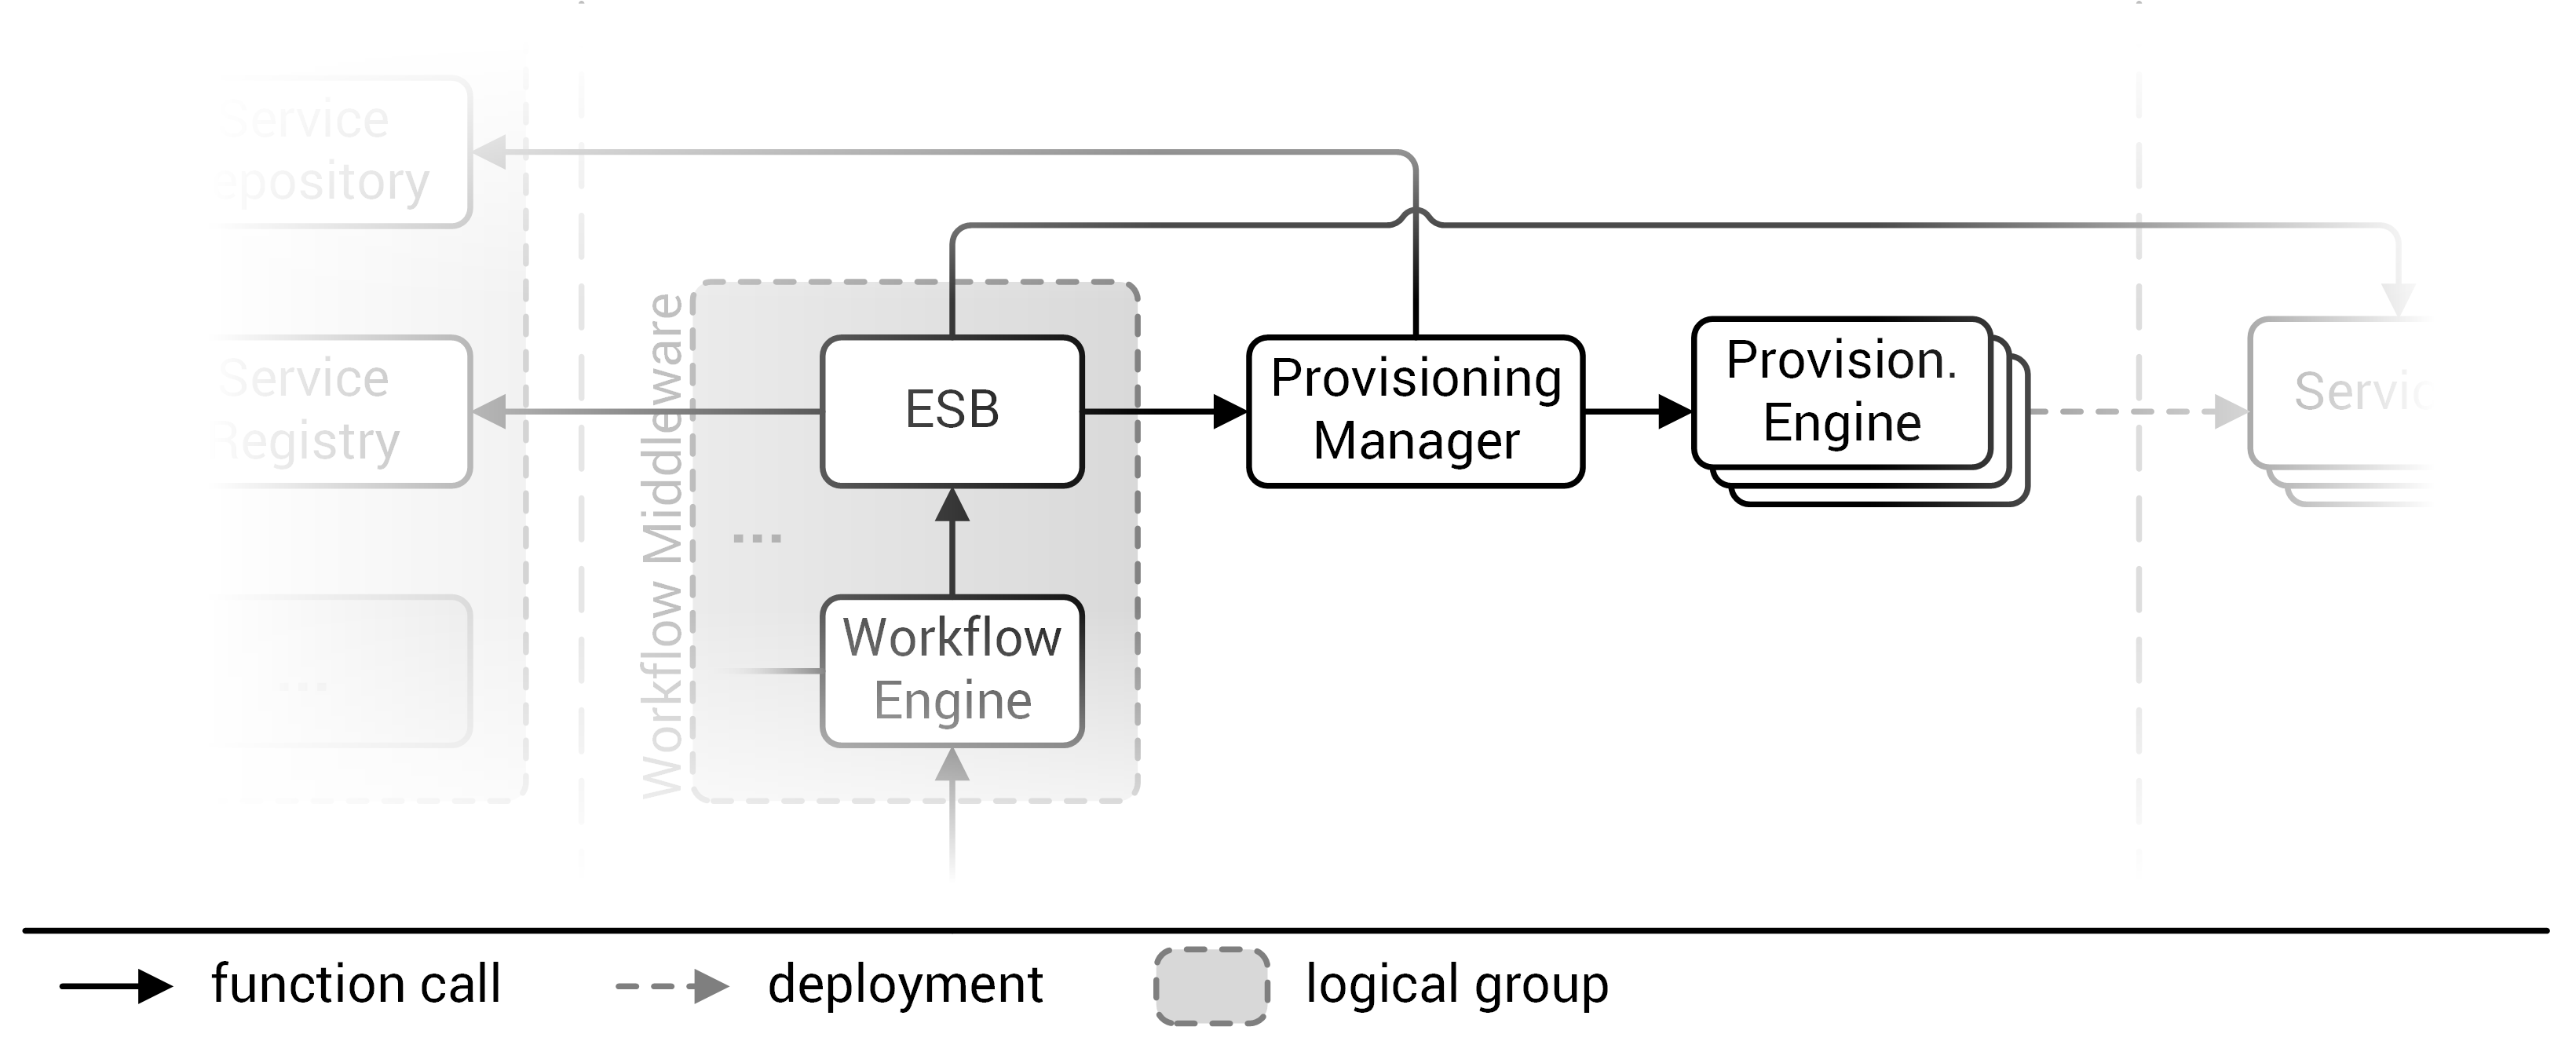
\includegraphics[resolution=600]{previous/assets/valeri_architecture}
	\caption{Extended architecture with added provisioning manager~\autocite[based on][]{serviceselection}.}
	\label{image:valeri_architecture}
\end{figure}

\citeauthor*{provisioning:dynamic} further refines the previously shown middleware architecture by adding a provisioning manager as intermediary between the ESB and the provisioning engines~\autocite{provisioning:dynamic}.
\autoref{image:valeri_architecture} shows an excerpt of the extended architecture with the additional provisioning manager at the center.
This addition improves the original architecture in three aspects.

The ESB can now use the stable interface of the provisioning manager to trigger provisioning engines instead of calling those provisioning engines directly.
The provisioning manager handles the differences between the provisioning engines.
This makes it also possible to use multiple different provisioning engines during one workflow execution.
The provisioning manager also handles the communication with the service repository or possibly multiple service repositories for different provisioning engines.
It can provide information to a particular provisioning engine if it cannot get the information it needs from the service repository on its own.
The provisioning manager could also translate different service distribution formats so that provisioning engines could be used with formats that they do not support~\autocite{provisioning:dynamic}.
